\section{Interconnessione di sistemi}

Possiamo modellizzare sistemi complessi costituiti dall'interazione di molti sistemi dinamici, a tale scopo risulta fondamentale comprendere come si struttura la connessione di più sistemi tra di loro.\\

Consideriamo una serie di \textbf{n} sistemi (\textbf{nodi}) che vogliamo collegare con una serie di \textbf{link} di lunghezza \textbf{d}. Se ogni nodo, che potrebbe per esempio essere la cellula di un organismo, ha una dimensione lineare \textbf{l} e il sistema totale, nel nostro esempio l'organismo, ha dimensione lineare \textbf{L} possiamo definire un \textbf{fattore di scala M} che stima quanti nodi sono presenti nel sistema quando il loro numero è nell'ordine della complessità:
\paragraph{Fattore di scala}
\begin{multicols}{2}
	\begin{center}
		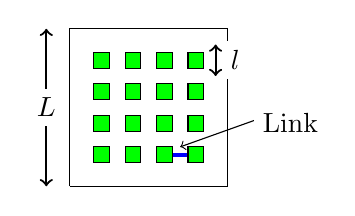
\begin{tikzpicture}
			\draw[step=0.1cm] (0.2,0) -- (0.2,2) -- (2.2,2) -- (2.2,0) -- (0.2,0);
			\draw[thick, <->] (-0.1,0) -- (-0.1,2);
			\node[fill=white] at (-0.1,1) {$L$};
			
			\draw[ultra thick,draw=blue] (1.4,0.4) -- (1.8,0.4);
			
			\filldraw[fill=green, draw=black] (0.5,0.3) rectangle (0.7,0.5);
			\filldraw[fill=green, draw=black] (0.9,0.3) rectangle (1.1,0.5);
			\filldraw[fill=green, draw=black] (1.3,0.3) rectangle (1.5,0.5);
			\filldraw[fill=green, draw=black] (1.7,0.3) rectangle (1.9,0.5);
			
			\filldraw[fill=green, draw=black] (0.5,0.7) rectangle (0.7,0.9);
			\filldraw[fill=green, draw=black] (0.9,0.7) rectangle (1.1,0.9);
			\filldraw[fill=green, draw=black] (1.3,0.7) rectangle (1.5,0.9);
			\filldraw[fill=green, draw=black] (1.7,0.7) rectangle (1.9,0.9);
			
			\filldraw[fill=green, draw=black] (0.5,1.1) rectangle (0.7,1.3);
			\filldraw[fill=green, draw=black] (0.9,1.1) rectangle (1.1,1.3);
			\filldraw[fill=green, draw=black] (1.3,1.1) rectangle (1.5,1.3);
			\filldraw[fill=green, draw=black] (1.7,1.1) rectangle (1.9,1.3);
			
			\filldraw[fill=green, draw=black] (0.5,1.5) rectangle (0.7,1.7);
			\filldraw[fill=green, draw=black] (0.9,1.5) rectangle (1.1,1.7);
			\filldraw[fill=green, draw=black] (1.3,1.5) rectangle (1.5,1.7);
			\filldraw[fill=green, draw=black] (1.7,1.5) rectangle (1.9,1.7);
			
			\draw[thick, <->] (2.05,1.4) -- (2.05,1.8);
			\node[fill=white] at (2.3,1.6) {$l$};
			
			\draw[ <-] (1.6,0.5) -- (3,1);
			\node[fill=white] at (3,0.81) {Link};
			
			
			
		\end{tikzpicture}
	
	\begin{equation}
		M=\left(\frac{L}{l}\right)^D \label{fattoreDiScalaInterconnessioni}
	\end{equation}
\end{center}
\end{multicols}
\vspace{20pt}
dove D è la dimensione del sistema (1D, 2D, 3D).\\

A questo punto possiamo iniziare a stimare il \textbf{costo} di una certa configurazione di link, ossia, se immaginiamo di trasportare un flusso $\Phi$, per esempio di energia o di corrente o di acqua, con il nostro sistema di link, quanto flusso è necessario perchè ogni nodo sia rifornito. \\
Supponiamo quindi che ad ogni nodo si impieghi una quantità $\phi$ di flusso e definiamo il costo del link i-esimo $d\cdot \phi$. Siamo a questo punto costretti ad analizzare l'esempio più semplice di rete per poter comprendere come avviene la sua analisi.

\subsection{Modello lineare}
\begin{center}
	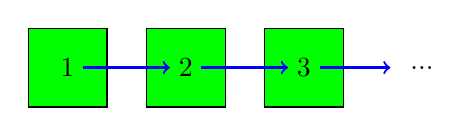
\begin{tikzpicture}
		\filldraw[fill=green,draw=black] (0,0) rectangle (1,1);
		\node[fill=green] at (0.5,0.5) {1};
		\filldraw[fill=green,draw=black] (1.5,0) rectangle (2.5,1);
		\node[fill=green] at (2,0.5) {2};
		\filldraw[fill=green,draw=black] (3,0) rectangle (4,1);
		\node[fill=green] at (3.5,0.5) {3};
		\draw[->,thick, draw=blue] (0.7,0.5) -- (1.8,0.5);
		\draw[->,thick, draw=blue] (2.2,0.5) -- (3.3,0.5);
		\draw[->,thick, draw=blue] (3.7,0.5) -- (4.6,0.5);
		\node[fill=white] at (5,0.5){...};
	\end{tikzpicture}\\
\end{center}



Immaginiamo di collegare ogni nodo uno dopo l'altro a catena, per quanto abbiamo detto il flusso all'i-esimo nodo sarà $\Phi_i=\Phi_{i-1}-d\cdot \phi$. Per cui se il numero di nodi è stimabile con M il costo totale sarà:
\begin{align*}
	\sum^M_{k=1} d\cdot \phi\cdot k = d\cdot \phi\cdot \sum^M_{k=1} k=\frac{M(M-1)}{2}d\cdot \phi\backsimeq\frac{d\cdot\phi}{2}M^2
\end{align*} 
che utilizzando la (\ref{fattoreDiScalaInterconnessioni}) e ricorando che $L^3$ è circa il volume del sistema, il nostro modello prevede che, nel caso in cui le dimensioni dei nodi e dei link non varino ma aumentino solamente il loro numero, il costo del sistema di interconnessione aumenta con il quadrato del volume del corpo.
\begin{equation}
	Costo=\frac{d\cdot\phi}{2\cdot l^6}V^2
\end{equation}

\subsection{Modello ad albero}
\begin{center}
	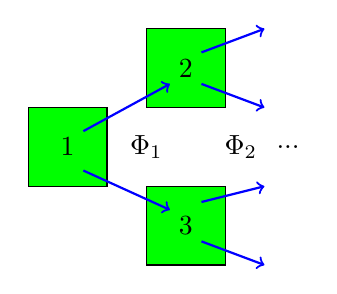
\begin{tikzpicture}
		\filldraw[fill=green,draw=black] (0,0) rectangle (1,1);
		\node[fill=green] at (0.5,0.5) {1};
		\filldraw[fill=green,draw=black] (1.5,1) rectangle (2.5,2);
		\node[fill=green] at (2,1.5) {2};
		\filldraw[fill=green,draw=black] (1.5,0) rectangle (2.5,-1);
		\node[fill=green] at (2,-0.5) {3};
		\draw[->,thick, draw=blue] (0.7,0.7) -- (1.8,1.3);
		\draw[->,thick, draw=blue] (0.7,0.2) -- (1.8,-0.3);
		\draw[->,thick, draw=blue] (2.2,1.7) -- (3,2);
		\draw[->,thick, draw=blue] (2.2,1.3) -- (3,1);
		\draw[->,thick, draw=blue] (2.2,-0.2) -- (3,0);
		\draw[->,thick, draw=blue] (2.2,-0.7) -- (3,-1);
		\node[fill=white] at (2.7,0.5) {$\Phi_2$};
		\node[fill=white] at (1.5,0.5) {$\Phi_1$};
		\node[fill=white] at (3.3,0.5){...};
	\end{tikzpicture}\\
\end{center}

In questo caso colleghiamo i nodi biforcando le connessioni ad ogni nodo in maniera tale che il flusso i-esimo risulti $\Phi_i=\frac{\Phi_{i-1}-\phi\cdot d}{2}$.

Questo sarebbe il comportamento ideale e più efficiente ma è possibile dimostrare che non è realizzabile.

\subsection{Modello a raggiera}
\begin{center}
	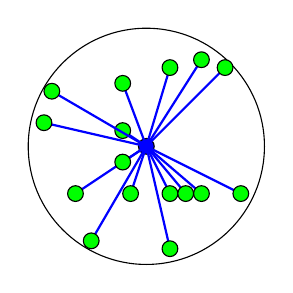
\begin{tikzpicture}
		\draw (0,0) circle (1.5cm);
		\filldraw[fill=blue] (0,0) circle (0.1cm);
		\draw[draw=blue, thick] (0,0) -- (1,1);
		\filldraw[fill=green] (1,1) circle (0.1cm);
		\draw[draw=blue, thick] (0,0) -- (0.3,-0.6);
		\filldraw[fill=green] (0.3,-0.6) circle (0.1cm);
		\draw[draw=blue, thick] (0,0) -- (-0.3,0.2);
		\filldraw[fill=green] (-0.3,0.2) circle (0.1cm);
		\draw[draw=blue, thick] (0,0) -- (-0.9,-0.6);
		\filldraw[fill=green] (-0.9,-0.6) circle (0.1cm);
		\draw[draw=blue, thick] (0,0) -- (0.3,1);
		\filldraw[fill=green] (0.3,1) circle (0.1cm);
		\draw[draw=blue, thick] (0,0) -- (0.7,-0.6);
		\filldraw[fill=green] (0.7,-0.6) circle (0.1cm);
		\draw[draw=blue, thick] (0,0) -- (-0.3,0.8);
		\filldraw[fill=green] (-0.3,0.8) circle (0.1cm);
		\draw[draw=blue, thick] (0,0) -- (-0.3,-0.2);
		\filldraw[fill=green] (-0.3,-0.2) circle (0.1cm);
		
		\draw[draw=blue, thick] (0,0) -- (-1.2,0.7);
		\filldraw[fill=green] (-1.2,0.7) circle (0.1cm);
		\draw[draw=blue, thick] (0,0) -- (1.2,-0.6);
		\filldraw[fill=green] (1.2,-0.6) circle (0.1cm);
		\draw[draw=blue, thick] (0,0) -- (0.7,1.1);
		\filldraw[fill=green] (0.7,1.1) circle (0.1cm);
		\draw[draw=blue, thick] (0,0) -- (-0.2,-0.6);
		\filldraw[fill=green] (-0.2,-0.6) circle (0.1cm);
		\draw[draw=blue, thick] (0,0) -- (0.3,-1.3);
		\filldraw[fill=green] (0.3,-1.3) circle (0.1cm);
		\draw[draw=blue, thick] (0,0) -- (0.5,-0.6);
		\filldraw[fill=green] (0.5,-0.6) circle (0.1cm);
		\draw[draw=blue, thick] (0,0) -- (-1.3,0.3);
		\filldraw[fill=green] (-1.3,0.3) circle (0.1cm);
		\draw[draw=blue, thick] (0,0) -- (-0.7,-1.2);
		\filldraw[fill=green] (-0.7,-1.2) circle (0.1cm);
		
	\end{tikzpicture}
\end{center}

Colleghiamo in questo caso ogni nodo con un singolo link, allora la lunghezza media dei link è confrontabile con la dimensione lineare del sistema per cui il costo è facilmente stimato come:
\begin{equation}
	Costo\ \sim M \phi L \sim \phi M^{\frac{D+1}{D}} 
\end{equation}
ricordando che $L^D\sim M$.\\

Osserviamo subito che in questo caso se il sistema si distribuisce linearmente o su una superficie, come una città, o nello spazio, come il corpo umano, questo modifica sensibilmente la forma analitica del costo. Infatti se $D=1$ otteniamo un dipendenza quadratica da $L$, mentre su una superficie abbiamo una dipendenza come $x^{\frac{3}{2}}$ dall'area occupata e per $D=3$ abbiamo:
\begin{equation}
	Costo\ \sim \phi V^{\frac{4}{3}} \label{modelloRaggieraTeorico}
\end{equation}

Questo modello si rivela essere il migliore sistema logistico realizzabile da un punto di vista teorico. In realtà però si scopre che non è il modello che la natura ha scelto per gli organismi viventi per esempio. 
\paragraph{Legge di Kleiber}
Si scopre infatti che la massa corporea, quindi il volume, di un organismo è legato alla potenza dissipata dal metabolismo basale da una legge a potenza nella forma:
\begin{equation}
	P\sim V^{\frac{3}{4}}
\end{equation}
che è molto differente dalla legge che abbiamo ricavato, il che ci suggerisce che la natura tiene conto anche di altri fattori per lo sviluppo delle reti logistiche negli organismi.